\chapter{全探索 - Complete search}

\key{全探索 - Complete search}は、
ほとんどすべてのアルゴリズムの問題を解決するために使用できる一般的な方法です。
ブルートフォースとも呼ばれ、問題に対して可能な限りの解を生成します。
完全探索は、すべての解を調べるのに十分な時間があればとても手法です。

なぜなら、この探索は通常、他の解法に比べて実装が簡単で、
常に正しい答えが得られるからです。
完全探索が遅すぎる場合は貪欲アルゴリズムや動的計画法など、
他の技法が必要になってくるでしょう。

\section{部分集合を全生成する - Generating subsets}

\index{部分集合 - subset}

$n$個の要素からなる集合のすべての部分集合を生成する問題を考えましょう。
例 えば$\{0,1,2\}$の部分集合は、
$\emptyset$, $\{0\}$, $\{1\}$, $\{2\}$, $\{0,1\}$,
$\{0,2\}$, $\{1,2\}$ and $\{0,1,2\}$です。
部分集合の生成には、再帰的探索を行う方法と、
整数のビット表現を利用する方法の2つが一般的です。

\subsubsection{Method 1}

集合のすべての部分集合を調べる1つ目の方法は再帰です。
次の関数 \texttt{search}は、集合 $\{0,1,\ldots,n-1\}$の部分集合を生成します。
この関数は、
各集合の要素を含むベクトル部分集合を保持します。
この探索はパラメ ータとして0を与えることで開始されます.

\begin{lstlisting}
void search(int k) {
    if (k == n) {
        // process subset
    } else {
        search(k+1);
        subset.push_back(k);
        search(k+1);
        subset.pop_back();
    }
}
\end{lstlisting}

関数\texttt{search}がパラメータ$k$で呼ばれると
要素$k$を部分集合に含めるかどうかを決定し、
いずれの場合もパラメータ$k + 1$で自分自身を呼び出します。
そして、$k = n$の場合,
関数はすべての要素が処理されて部分集合が生成されたとして終わります。
次のツリーは、$n = 3$ のときの関数呼び出しを示したものです。
左の枝($k$ は部分集合に含まれない)と右の枝($k$は部分集合に含まれる)のどちらが常に選ばれます。

\begin{center}
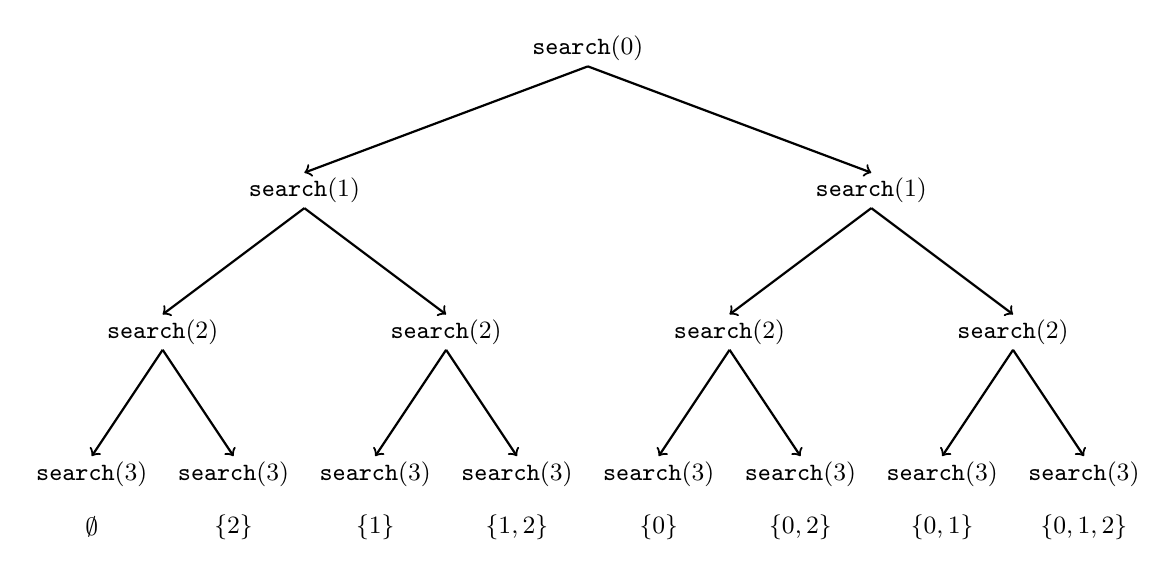
\begin{tikzpicture}[scale=.45]
  \begin{scope}
    \small
    \node at (0,0) {$\texttt{search}(0)$};

    \node at (-8,-4) {$\texttt{search}(1)$};
    \node at (8,-4) {$\texttt{search}(1)$};

    \path[draw,thick,->] (0,0-0.5) -- (-8,-4+0.5);
    \path[draw,thick,->] (0,0-0.5) -- (8,-4+0.5);

    \node at (-12,-8) {$\texttt{search}(2)$};
    \node at (-4,-8) {$\texttt{search}(2)$};
    \node at (4,-8) {$\texttt{search}(2)$};
    \node at (12,-8) {$\texttt{search}(2)$};

    \path[draw,thick,->] (-8,-4-0.5) -- (-12,-8+0.5);
    \path[draw,thick,->] (-8,-4-0.5) -- (-4,-8+0.5);
    \path[draw,thick,->] (8,-4-0.5) -- (4,-8+0.5);
    \path[draw,thick,->] (8,-4-0.5) -- (12,-8+0.5);

    \node at (-14,-12) {$\texttt{search}(3)$};
    \node at (-10,-12) {$\texttt{search}(3)$};
    \node at (-6,-12) {$\texttt{search}(3)$};
    \node at (-2,-12) {$\texttt{search}(3)$};
    \node at (2,-12) {$\texttt{search}(3)$};
    \node at (6,-12) {$\texttt{search}(3)$};
    \node at (10,-12) {$\texttt{search}(3)$};
    \node at (14,-12) {$\texttt{search}(3)$};

    \node at (-14,-13.5) {$\emptyset$};
    \node at (-10,-13.5) {$\{2\}$};
    \node at (-6,-13.5) {$\{1\}$};
    \node at (-2,-13.5) {$\{1,2\}$};
    \node at (2,-13.5) {$\{0\}$};
    \node at (6,-13.5) {$\{0,2\}$};
    \node at (10,-13.5) {$\{0,1\}$};
    \node at (14,-13.5) {$\{0,1,2\}$};


    \path[draw,thick,->] (-12,-8-0.5) -- (-14,-12+0.5);
    \path[draw,thick,->] (-12,-8-0.5) -- (-10,-12+0.5);
    \path[draw,thick,->] (-4,-8-0.5) -- (-6,-12+0.5);
    \path[draw,thick,->] (-4,-8-0.5) -- (-2,-12+0.5);
    \path[draw,thick,->] (4,-8-0.5) -- (2,-12+0.5);
    \path[draw,thick,->] (4,-8-0.5) -- (6,-12+0.5);
    \path[draw,thick,->] (12,-8-0.5) -- (10,-12+0.5);
    \path[draw,thick,->] (12,-8-0.5) -- (14,-12+0.5);
\end{scope}
\end{tikzpicture}
\end{center}

\subsubsection{Method 2}

部分集合を生成するもう一つの方法は、ビット列を使う方法です。
$n$個の要素からなる集合のそれぞれの部分集合は$0 \ldots 2^n-1$
の間の整数に対 応する$n$ビット列として表現できます。
1は、どの要素が部分集合に含まれるかを示す。
一般的な実装では最後のビットが要素0に対応し、
2番目のビットが要素1に対応し..となります。
例えば、25のビット表現は11001でですが、これは部分集合$\{0,3,4\}$に対応します。

次のコードは、$n$個の要素を持つ集合の部分集合を調べます

\begin{lstlisting}
for (int b = 0; b < (1<<n); b++) {
    // process subset
}
\end{lstlisting}

次のコードは、ビット列に対応する部分集合の要素を見つける方法です。
各部分集合を処理するとき、コードはサブセットの要素を含むベクトルを返します。

\begin{lstlisting}
for (int b = 0; b < (1<<n); b++) {
    vector<int> subset;
    for (int i = 0; i < n; i++) {
        if (b&(1<<i)) subset.push_back(i);
    }
}
\end{lstlisting}

\section{順列の生成 - Generating permutations}

\index{順列 - permutation}

$n$個の要素からなる集合のすべての並べ換えを生成する問題を考えましょう。
例えば,$\{0,1,2\}$の並べ換えは,
$(0,1,2)$, $(0,2,1)$, $(1,0,2)$, $(1,2,0)$,
$(2,0,1)$, $(2,1,0)$です。
ここでも2つのアプローチがあります。再帰を使うか、順列を繰り返し見ていくかのどちらかである。

\subsubsection{Method 1}

並べ換えも再帰を使って生成できます。
次の関数\texttt{search}は、
集合  $\{0,1,\ldots,n-1\}$ の並べ換えを列挙します。
この関数は、並べ換えを含むベクターを構築し、
パラメータなしでこの関数が呼ばれたときに探索が開始されます。

\begin{lstlisting}
void search() {
    if (permutation.size() == n) {
        // process permutation
    } else {
        for (int i = 0; i < n; i++) {
            if (chosen[i]) continue;
            chosen[i] = true;
            permutation.push_back(i);
            search();
            chosen[i] = false;
            permutation.pop_back();
        }
    }
}
\end{lstlisting}

関数呼び出しのたび、新しいエレメントが
\texttt{permutation}
に追加されます。
配列\texttt{chosen} はどの要素がすでに入ったかを格納します。
そして、\texttt{permutation}の長さが求めたいものと一致した時に、
それを結果とします。

\subsubsection{Method 2}

\index{next\_permutation@\texttt{next\_permutation}}

もう一つの方法は、この順列を
$\{0,1,\ldots,n-1\}$ から開始することです。
そして、次の順列、を求めていくことです。
C++の標準ライブラリにはこのための関数
\texttt{next\_permutation} があり、次のように使うことができます。

\begin{lstlisting}
vector<int> permutation;
for (int i = 0; i < n; i++) {
    permutation.push_back(i);
}
do {
    // process permutation
} while (next_permutation(permutation.begin(),permutation.end()));
\end{lstlisting}

\section{バックトラッキング - Backtracking}

\index{バックトラッキング - backtracking}

\key{バックトラッキング - backtracking} のアルゴリズムとは、
空の解から始まり、
段階的に解を作っていきます。探索は、解がどのように構築されうるかを
再帰で全探索していきます。

\index{クイーン問題 - queen problem}

例えば、$n \times n$ のチェス盤の上に、
2つの女王が互いに攻撃し合わないように、
$n$個の女王を配置する方法の数を計算する問題を考えます。これは、クイーン問題として知られています。
例えば 、$n=4$のとき、2つの解が考えられる。

\begin{center}
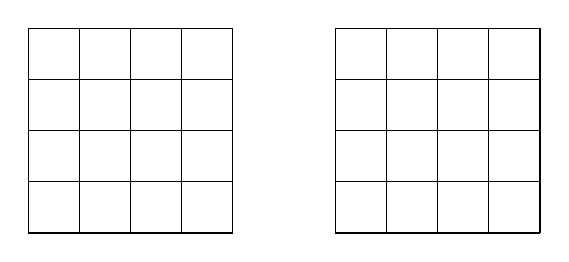
\begin{tikzpicture}[scale=.65]
  \begin{scope}
    \draw (0, 0) grid (4, 4);
    \node at (1.5,3.5) {\symqueen};
    \node at (3.5,2.5) {\symqueen};
    \node at (0.5,1.5) {\symqueen};
    \node at (2.5,0.5) {\symqueen};

    \draw (6, 0) grid (10, 4);
    \node at (6+2.5,3.5) {\symqueen};
    \node at (6+0.5,2.5) {\symqueen};
    \node at (6+3.5,1.5) {\symqueen};
    \node at (6+1.5,0.5) {\symqueen};

  \end{scope}
\end{tikzpicture}
\end{center}

クイーン問題は、バックトラックを使用して、
ボードに一列ずつクイーンを配置することで解くことができます。
各ターンでは、それまでに置かれたクイーンを攻撃するクイーンがないように、
各列にちょうど1つずつクイーンを置いていきます。
$n$個のクイーンがすべてボード上に配置されたときに解が得られます。

例えば、$n = 4$の場合、バックトラックアルゴリズムで生成される部分解は
以下のようになります。

\begin{center}
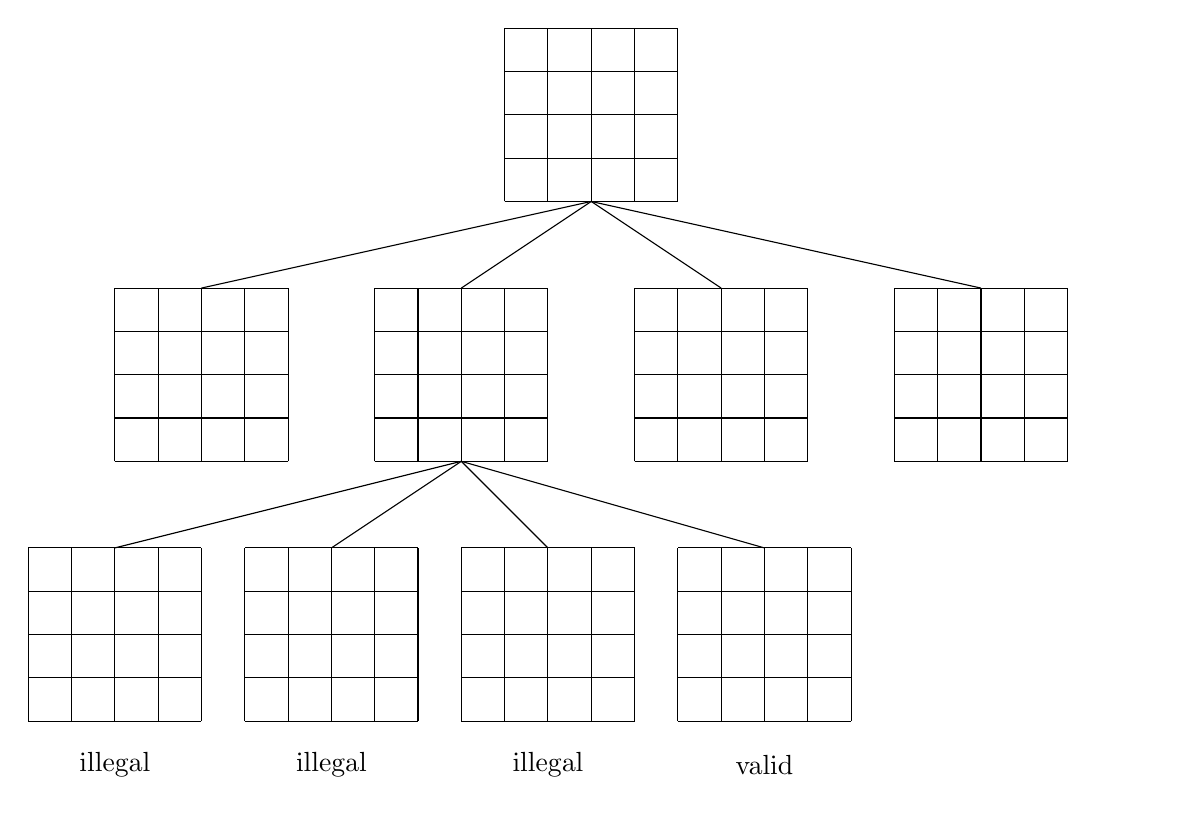
\begin{tikzpicture}[scale=.55]
  \begin{scope}
    \draw (0, 0) grid (4, 4);

    \draw (-9, -6) grid (-5, -2);
    \draw (-3, -6) grid (1, -2);
    \draw (3, -6) grid (7, -2);
    \draw (9, -6) grid (13, -2);

    \node at (-9+0.5,-3+0.5) {\symqueen};
    \node at (-3+1+0.5,-3+0.5) {\symqueen};
    \node at (3+2+0.5,-3+0.5) {\symqueen};
    \node at (9+3+0.5,-3+0.5) {\symqueen};

    \draw (2,0) -- (-7,-2);
    \draw (2,0) -- (-1,-2);
    \draw (2,0) -- (5,-2);
    \draw (2,0) -- (11,-2);

    \draw (-11, -12) grid (-7, -8);
    \draw (-6, -12) grid (-2, -8);
    \draw (-1, -12) grid (3, -8);
    \draw (4, -12) grid (8, -8);
    \draw[white] (11, -12) grid (15, -8);
    \node at (-11+1+0.5,-9+0.5) {\symqueen};
    \node at (-6+1+0.5,-9+0.5) {\symqueen};
    \node at (-1+1+0.5,-9+0.5) {\symqueen};
    \node at (4+1+0.5,-9+0.5) {\symqueen};
    \node at (-11+0+0.5,-10+0.5) {\symqueen};
    \node at (-6+1+0.5,-10+0.5) {\symqueen};
    \node at (-1+2+0.5,-10+0.5) {\symqueen};
    \node at (4+3+0.5,-10+0.5) {\symqueen};

    \draw (-1,-6) -- (-9,-8);
    \draw (-1,-6) -- (-4,-8);
    \draw (-1,-6) -- (1,-8);
    \draw (-1,-6) -- (6,-8);

    \node at (-9,-13) {illegal};
    \node at (-4,-13) {illegal};
    \node at (1,-13) {illegal};
    \node at (6,-13) {valid};

  \end{scope}
\end{tikzpicture}
\end{center}


下に示した最初の3つは、クイーン同士が攻撃しあっているので、不正な構成です。
しかし、4番目の構成は有効で、
さらに2つのクイーンをボードに配置することで完全な解答に拡張することができます。
なお、残りの2つのクイーンを配置する方法は1つだけです。

\begin{samepage}
これは次のように実装することができます。
\begin{lstlisting}
void search(int y) {
    if (y == n) {
        count++;
        return;
    }
    for (int x = 0; x < n; x++) {
        if (column[x] || diag1[x+y] || diag2[x-y+n-1]) continue;
        column[x] = diag1[x+y] = diag2[x-y+n-1] = 1;
        search(y+1);
        column[x] = diag1[x+y] = diag2[x-y+n-1] = 0;
    }
}
\end{lstlisting}
\end{samepage}

\texttt{search(0)}.を呼び出ししてこの探索は開始されます。
盤の大きさは  $n \times n$ であ、コードは数えるべき解の数を計算します。

さて、このコードでは、盤面の行と列は0 to $n-1$までの番号が付けられているとします。
関数\texttt{search}がパラメータ$y$で呼ばれると、
$y$行にクイーンを置き、
内部ではパラメータ$y + 1$で自分自身を呼び出します。
そして、$y = n$ ならば、解が見つかったことになり、\texttt{count} が1つ増加します。

配列\texttt{column} はクイーンを含む列を、
配列\texttt{diag1}および\texttt{diag2}は対角線を追跡します。
すでにクイーンを含む列や対角線に、さらにクイーンを追加することはできません。
例えば、$4 \times 4$ のボードの列と対角線は次のように番号付けされています。

\begin{center}
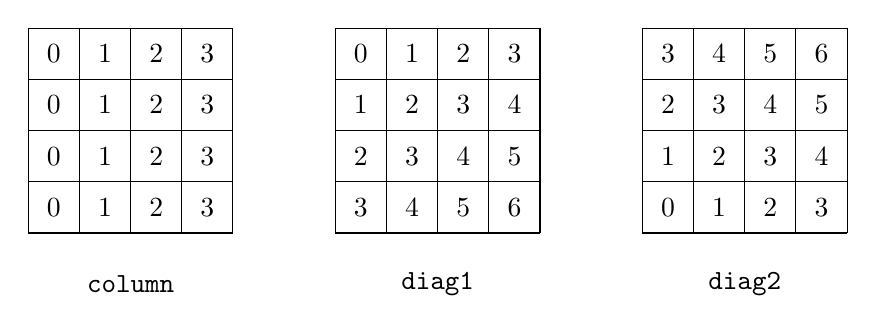
\begin{tikzpicture}[scale=.65]
  \begin{scope}
    \draw (0-6, 0) grid (4-6, 4);
    \node at (-6+0.5,3.5) {$0$};
    \node at (-6+1.5,3.5) {$1$};
    \node at (-6+2.5,3.5) {$2$};
    \node at (-6+3.5,3.5) {$3$};
    \node at (-6+0.5,2.5) {$0$};
    \node at (-6+1.5,2.5) {$1$};
    \node at (-6+2.5,2.5) {$2$};
    \node at (-6+3.5,2.5) {$3$};
    \node at (-6+0.5,1.5) {$0$};
    \node at (-6+1.5,1.5) {$1$};
    \node at (-6+2.5,1.5) {$2$};
    \node at (-6+3.5,1.5) {$3$};
    \node at (-6+0.5,0.5) {$0$};
    \node at (-6+1.5,0.5) {$1$};
    \node at (-6+2.5,0.5) {$2$};
    \node at (-6+3.5,0.5) {$3$};

    \draw (0, 0) grid (4, 4);
    \node at (0.5,3.5) {$0$};
    \node at (1.5,3.5) {$1$};
    \node at (2.5,3.5) {$2$};
    \node at (3.5,3.5) {$3$};
    \node at (0.5,2.5) {$1$};
    \node at (1.5,2.5) {$2$};
    \node at (2.5,2.5) {$3$};
    \node at (3.5,2.5) {$4$};
    \node at (0.5,1.5) {$2$};
    \node at (1.5,1.5) {$3$};
    \node at (2.5,1.5) {$4$};
    \node at (3.5,1.5) {$5$};
    \node at (0.5,0.5) {$3$};
    \node at (1.5,0.5) {$4$};
    \node at (2.5,0.5) {$5$};
    \node at (3.5,0.5) {$6$};

    \draw (6, 0) grid (10, 4);
    \node at (6.5,3.5) {$3$};
    \node at (7.5,3.5) {$4$};
    \node at (8.5,3.5) {$5$};
    \node at (9.5,3.5) {$6$};
    \node at (6.5,2.5) {$2$};
    \node at (7.5,2.5) {$3$};
    \node at (8.5,2.5) {$4$};
    \node at (9.5,2.5) {$5$};
    \node at (6.5,1.5) {$1$};
    \node at (7.5,1.5) {$2$};
    \node at (8.5,1.5) {$3$};
    \node at (9.5,1.5) {$4$};
    \node at (6.5,0.5) {$0$};
    \node at (7.5,0.5) {$1$};
    \node at (8.5,0.5) {$2$};
    \node at (9.5,0.5) {$3$};

    \node at (-4,-1) {\texttt{column}};
    \node at (2,-1) {\texttt{diag1}};
    \node at (8,-1) {\texttt{diag2}};

  \end{scope}
\end{tikzpicture}
\end{center}


$n \times n$ のチェス盤に $n$ 個のクイーンを配置する方法の数を $q(n)$ としましょう。
上記のバックトラックアルゴリズムにより、例えば、$q(8)=92$となることがわかります。
$n$が大きくなると、解の数は指数関数的に増えるので、探索はすぐに遅くなってしまいます。
例えば、 上記のアルゴリズムを使って$q(16)=14772512$を計算すると、
最新のコンピュータでも1分以上かかります。\footnote{There is no known way to efficiently
calculate larger values of $q(n)$. The current record is
$q(27)=234907967154122528$, calculated in 2016 \cite{q27}.}.

\section{枝刈り - Pruning the search}

バックトラックを探索木の枝刈りで最適化することができる場合が多いです。
このアイデアは、アルゴリズムに''intelligence''を加えることで、
部分解が完全解に拡張できない場合、できるだけ早くそれに気づきその先の探索をやめます。
このような最適化は、探索の効率に多大な影響を与える。

ここで、$n \times n$ の格子において、
左上から右下に向かう経路が各マスをちょうど1回ずつ訪れるような経路の数を計算する問題を考えてみましょう。
例えば、$7 \times 7$ のマス目では、
111712本のパスが存在します。
例として、そのうちの1本は次のようなものです。

\begin{center}
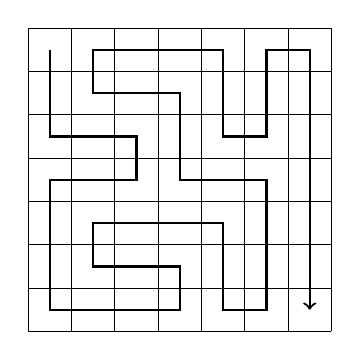
\begin{tikzpicture}[scale=.55]
  \begin{scope}
    \draw (0, 0) grid (7, 7);
    \draw[thick,->] (0.5,6.5) -- (0.5,4.5) -- (2.5,4.5) --
          (2.5,3.5) -- (0.5,3.5) -- (0.5,0.5) --
          (3.5,0.5) -- (3.5,1.5) -- (1.5,1.5) --
          (1.5,2.5) -- (4.5,2.5) -- (4.5,0.5) --
          (5.5,0.5) -- (5.5,3.5) -- (3.5,3.5) --
          (3.5,5.5) -- (1.5,5.5) -- (1.5,6.5) --
          (4.5,6.5) -- (4.5,4.5) -- (5.5,4.5) --
          (5.5,6.5) -- (6.5,6.5) -- (6.5,0.5);
  \end{scope}
\end{tikzpicture}
\end{center}

$7 \times 7$のケースは難易度が高く、我々のニーズに合っているため、
このケース を取り上げることにします。
まず、素直なバックトラックアルゴリズムから始め 、
探索をどのように刈り込むことができるかの観察を用いて、
段階的に最適化する方法を見ていきます。
各最適化の後、アルゴリズムの実行時間と再帰呼び出しの数を測定し、
各最適化がどのような影響を与えたのかを調べてみましょう。

\subsubsection{基本的なアルゴリズム - Basic algorithm}

最初のバージョンのアルゴリズムは最適化をせずに
単にバックトラックを使って、左上隅から右下隅への可能な経路をすべて生成し、
そのような経路の数をカウントします。

\begin{itemize}
\item
running time: 483 秒
\item
number of recursive calls: 760 億回
\end{itemize}

\subsubsection{最適化1 - Optimization 1}

どの解法でも、必ず1段下か右に移動します。
最初のステップの後、グリッドの対角線に関して対称な2つのパスが必ず存在します。
例えば、次のような経路です。

\begin{center}
\begin{tabular}{ccc}
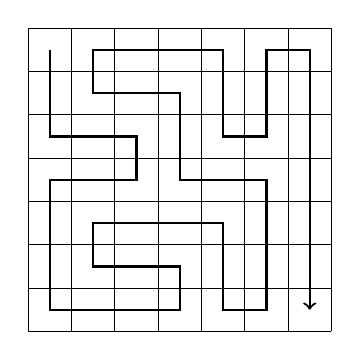
\begin{tikzpicture}[scale=.55]
  \begin{scope}
    \draw (0, 0) grid (7, 7);
    \draw[thick,->] (0.5,6.5) -- (0.5,4.5) -- (2.5,4.5) --
          (2.5,3.5) -- (0.5,3.5) -- (0.5,0.5) --
          (3.5,0.5) -- (3.5,1.5) -- (1.5,1.5) --
          (1.5,2.5) -- (4.5,2.5) -- (4.5,0.5) --
          (5.5,0.5) -- (5.5,3.5) -- (3.5,3.5) --
          (3.5,5.5) -- (1.5,5.5) -- (1.5,6.5) --
          (4.5,6.5) -- (4.5,4.5) -- (5.5,4.5) --
          (5.5,6.5) -- (6.5,6.5) -- (6.5,0.5);
  \end{scope}
\end{tikzpicture}
& \hspace{20px}
& 
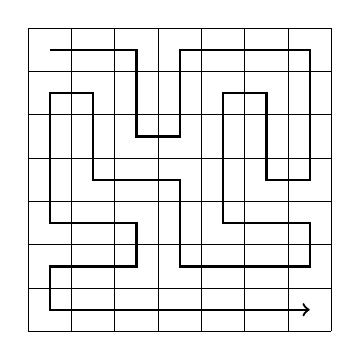
\begin{tikzpicture}[scale=.55]
  \begin{scope}[yscale=1,xscale=-1,rotate=-90]
    \draw (0, 0) grid (7, 7);
    \draw[thick,->] (0.5,6.5) -- (0.5,4.5) -- (2.5,4.5) --
          (2.5,3.5) -- (0.5,3.5) -- (0.5,0.5) --
          (3.5,0.5) -- (3.5,1.5) -- (1.5,1.5) --
          (1.5,2.5) -- (4.5,2.5) -- (4.5,0.5) --
          (5.5,0.5) -- (5.5,3.5) -- (3.5,3.5) --
          (3.5,5.5) -- (1.5,5.5) -- (1.5,6.5) --
          (4.5,6.5) -- (4.5,4.5) -- (5.5,4.5) --
          (5.5,6.5) -- (6.5,6.5) -- (6.5,0.5);
  \end{scope}
\end{tikzpicture}
\end{tabular}
\end{center}

つまり、まず必ず1段階下(または右)に移動したあとの解の数から2倍する、とできます。

\begin{itemize}
\item
running time: 244 秒
\item
number of recursive calls: 380 億回
\end{itemize}

\subsubsection{最適化2 - Optimization 2}

もし、他のマスをすべて訪問する前に右下のマスに到達した場合、
完成させることができないことは明らかです。

\begin{center}
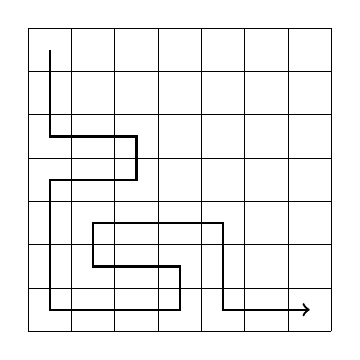
\begin{tikzpicture}[scale=.55]
  \begin{scope}
    \draw (0, 0) grid (7, 7);
    \draw[thick,->] (0.5,6.5) -- (0.5,4.5) -- (2.5,4.5) --
          (2.5,3.5) -- (0.5,3.5) -- (0.5,0.5) --
          (3.5,0.5) -- (3.5,1.5) -- (1.5,1.5) --
          (1.5,2.5) -- (4.5,2.5) -- (4.5,0.5) --
          (6.5,0.5);
  \end{scope}
\end{tikzpicture}
\end{center}

これを用いて早く右下に到達した探索は打ち切ることにします。

\begin{itemize}
\item
running time: 119 秒
\item
number of recursive calls: 200億回
\end{itemize}

\subsubsection{Optimization 3}

パスが壁に接触して左右に曲がることができるような場合、
グリッドは未訪問のマスを含む2つの部分に分割されます。
次のような場合、道は左にも右にも曲がることができます。

\begin{center}
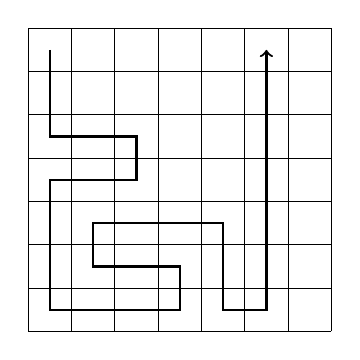
\begin{tikzpicture}[scale=.55]
  \begin{scope}
    \draw (0, 0) grid (7, 7);
    \draw[thick,->] (0.5,6.5) -- (0.5,4.5) -- (2.5,4.5) --
          (2.5,3.5) -- (0.5,3.5) -- (0.5,0.5) --
          (3.5,0.5) -- (3.5,1.5) -- (1.5,1.5) --
          (1.5,2.5) -- (4.5,2.5) -- (4.5,0.5) --
          (5.5,0.5) -- (5.5,6.5);
  \end{scope}
\end{tikzpicture}
\end{center}

このシチュエーションはどちらを選んだとしても、
もうすべてのマスを訪問することはできないので探索を打ち切ります。
この最適化は非常に有効です。


\begin{itemize}
\item
running time: 1.8 秒
\item
number of recursive calls: 2億2100万回
\end{itemize}

\subsubsection{最適化4 - Optimization 4}

最適化3の考え方は壁に当たった時以外にも一般化することができます。
もし、パスが前に進むことができず、左か右に曲がることができる場合、
グリッドは2つに分かれてしまうので未訪問のマスを含むことになります。
例えば、次のような経路がこれにあたります。

The idea of Optimization 3
can be generalized:
if the path cannot continue forward
but can turn either left or right,
the grid splits into two parts
that both contain unvisited squares.
For example, consider the following path:

\begin{center}
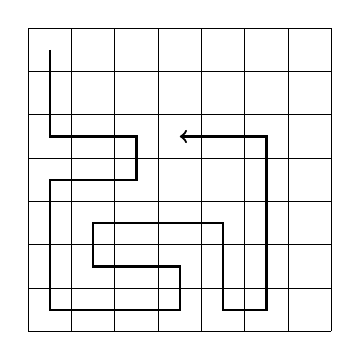
\begin{tikzpicture}[scale=.55]
  \begin{scope}
    \draw (0, 0) grid (7, 7);
    \draw[thick,->] (0.5,6.5) -- (0.5,4.5) -- (2.5,4.5) --
          (2.5,3.5) -- (0.5,3.5) -- (0.5,0.5) --
          (3.5,0.5) -- (3.5,1.5) -- (1.5,1.5) --
          (1.5,2.5) -- (4.5,2.5) -- (4.5,0.5) --
          (5.5,0.5) -- (5.5,4.5) -- (3.5,4.5);
  \end{scope}
\end{tikzpicture}
\end{center}

このようなケースも打ち切ると非常に効果的な探索が行えます。

\begin{itemize}
\item
running time: 0.6 秒
\item
number of recursive calls: 6900万回
\end{itemize}

~\\
さて、アルゴリズムの最適化はここまでにして成果を確認しましょう。
元のアルゴリズムの実行時間は483秒でしたが、最適化後の実行時間はわずか0.6秒 になりました。
このように、最適化によってアルゴリズムは1000倍近く高速化されました。

これはバックトラックによくあることで、
探索木は何もしなければ通常大きく、簡単な観察を活用するだけで効果的に
探索を刈り込むことができます。
特に有用なのは、アルゴリズムの最初ほうのステップ、すなわち、ツリーの上の方の枝刈りです。

\section{Meet in the middle}

\index{meet in the middle}

\key{Meet in the middle}は、
探索空間をほぼ同じ大きさの2つのパートに分割する手法のことです。
それぞれの部分に対して別々の検索を行い、最終的に検索結果を結合します。

検索結果を効率的に組み合わせる方法があれば、この手法を使うことができます。
そのような状況では、2つの検索は1つの大きな検索よりも短い時間で済むかもしれません。
典型的な例としては、meet in the middleのテクニックを使って、
ファクター $2^n$ をファクター$2^{n/2}$にすることができます。

例えば、$n$個の数字のリストとある数$x$が与えられたとき、
それらの和が$x$になるようなリストの中からいくつかの数字を選び方が可能かどうかを調べる問題を考えてみましょう。
例えば、リスト$[2,4,5,9]$と $x = 15$が与えられたとき 、
$[2,4,9]$ の数字を選べば、$2+4+9=15$になります。
しかし、同じリストに対して$x=10$とすると不可能です。

この問題に対する単純なアルゴリズムは、
要素のすべての部分集合を調べて、
いずれかの部分集合の和が$x$であるかどうかをチェックする方法です。
このようなアルゴリズムの実行時間は、$2^n$の部分集合を持つので
$O(2^{n/2})$ です。
で ある。しかし、meet in the middleの手法を用いると、より効率な$O(2^{n/2})$で求めることができます。
\footnote{This
idea was introduced in 1974 by E. Horowitz and S. Sahni \cite{hor74}.}.

ここで $O(2^n)$ と $O(2^{n/2})$ の時間計算量は全く異なることに注意します。
なぜなら、$2^{n/2}$ は $\sqrt{2^n}$に等しいです。

まず、リストを2つのリスト$A$、$B$に分割し、
両方のリストに約半分の数字が含まれるようにします。最初の検索では、
$A$のすべての部分集合を生成し、その和をリスト$S_A$に格納します。
同じようにリスト$B$からリスト$S_B$を作成します。
このあと、$S_A$と$S_B$からひとつずつ選び
それらの和が$x$になるようにできるかどうかを調べればよいです。
これは、元のリストの数を用いて和$x$を形成する方法がある場合に、まさに有効です。

例えば、リストが[2, 4, 5, 9]でx=15だとする。まず、リストをA=[2, 4]と B=[5, 9]に分割する。この後、リストSA = [0, 2, 4, 6]とSB = [0, 5, 9, 14]を作成し ます。この場合、SA には和 6 が、SB には和 9 が含まれ、6 + 9 = 15 となるので 、和 x = 15 を形成することが可能である。これは次のように対応する。 を解決することができます[2, 4, 9]。

このアルゴリズムは、その時間計算量がO(2n/2 )となるように実装することが できる。まず、ソートされたリストSA とSB を生成する。これは、マージのよ うな技法を用いてO(2n/2 ) 時間で行うことができる。この後、リストはソート されているので、SA と SB から和 x が生成できるかどうかを O(2n/2 ) 時間で確 認することができる。

The idea is to divide the list into
two lists $A$ and $B$ such that both
lists contain about half of the numbers.
The first search generates all subsets
of $A$ and stores their sums to a list $S_A$.
Correspondingly, the second search creates
a list $S_B$ from $B$.
After this, it suffices to check if it is possible
to choose one element from $S_A$ and another
element from $S_B$ such that their sum is $x$.
This is possible exactly when there is a way to
form the sum $x$ using the numbers of the original list.

For example, suppose that the list is $[2,4,5,9]$ and $x=15$.
First, we divide the list into $A=[2,4]$ and $B=[5,9]$.
After this, we create lists
$S_A=[0,2,4,6]$ and $S_B=[0,5,9,14]$.
In this case, the sum $x=15$ is possible to form,
because $S_A$ contains the sum $6$,
$S_B$ contains the sum $9$, and $6+9=15$.
This corresponds to the solution $[2,4,9]$.

We can implement the algorithm so that
its time complexity is $O(2^{n/2})$.
First, we generate \emph{sorted} lists $S_A$ and $S_B$,
which can be done in $O(2^{n/2})$ time using a merge-like technique.
After this, since the lists are sorted,
we can check in $O(2^{n/2})$ time if
the sum $x$ can be created from $S_A$ and $S_B$.